\subsection{Summary of the Changes to the Bifurcation Structure}

This section summarizes all the changes that happen to the \gls{pi} structure of the archetypal model when the parameters are changed in such a way that \gls{pal} structures emerge.
Furthermore, it provides an explanation for why the \gls{pi} structure of the archetypal model is impossible with only increasing branches.

\subsubsection{Schematics and Summary of the Changes}

\begin{figure}
	\centering
	\subfloat[]{
		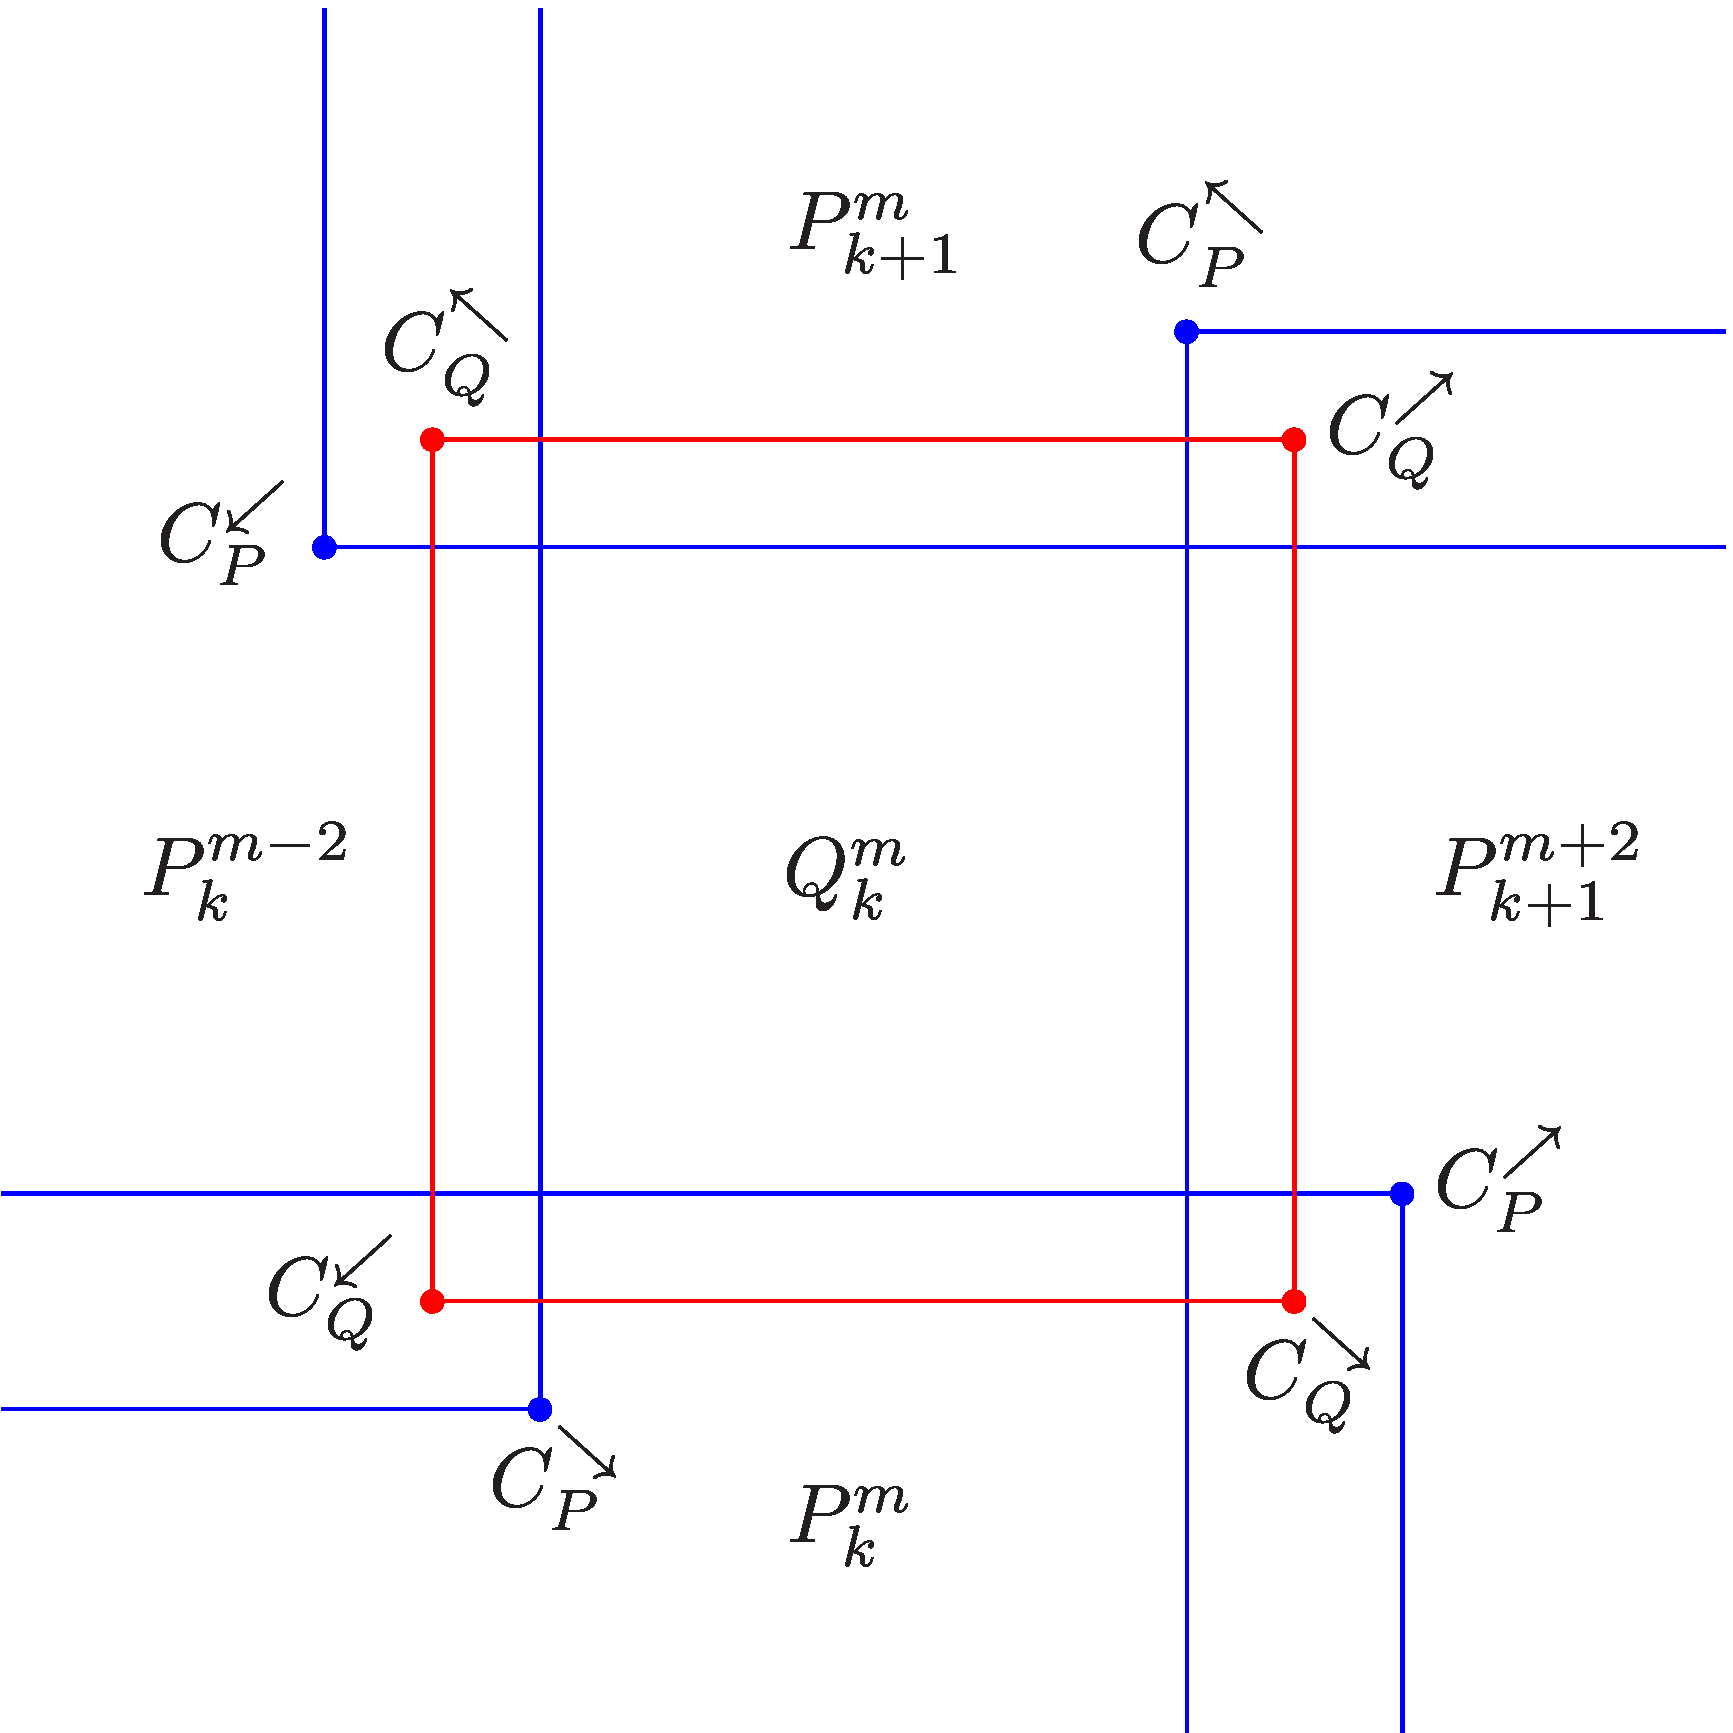
\includegraphics[width=.4 \textwidth]{../Figures/7/7.9a/result.png}
		\label{fig:add.change.schema.a}
	}
	\subfloat[]{
		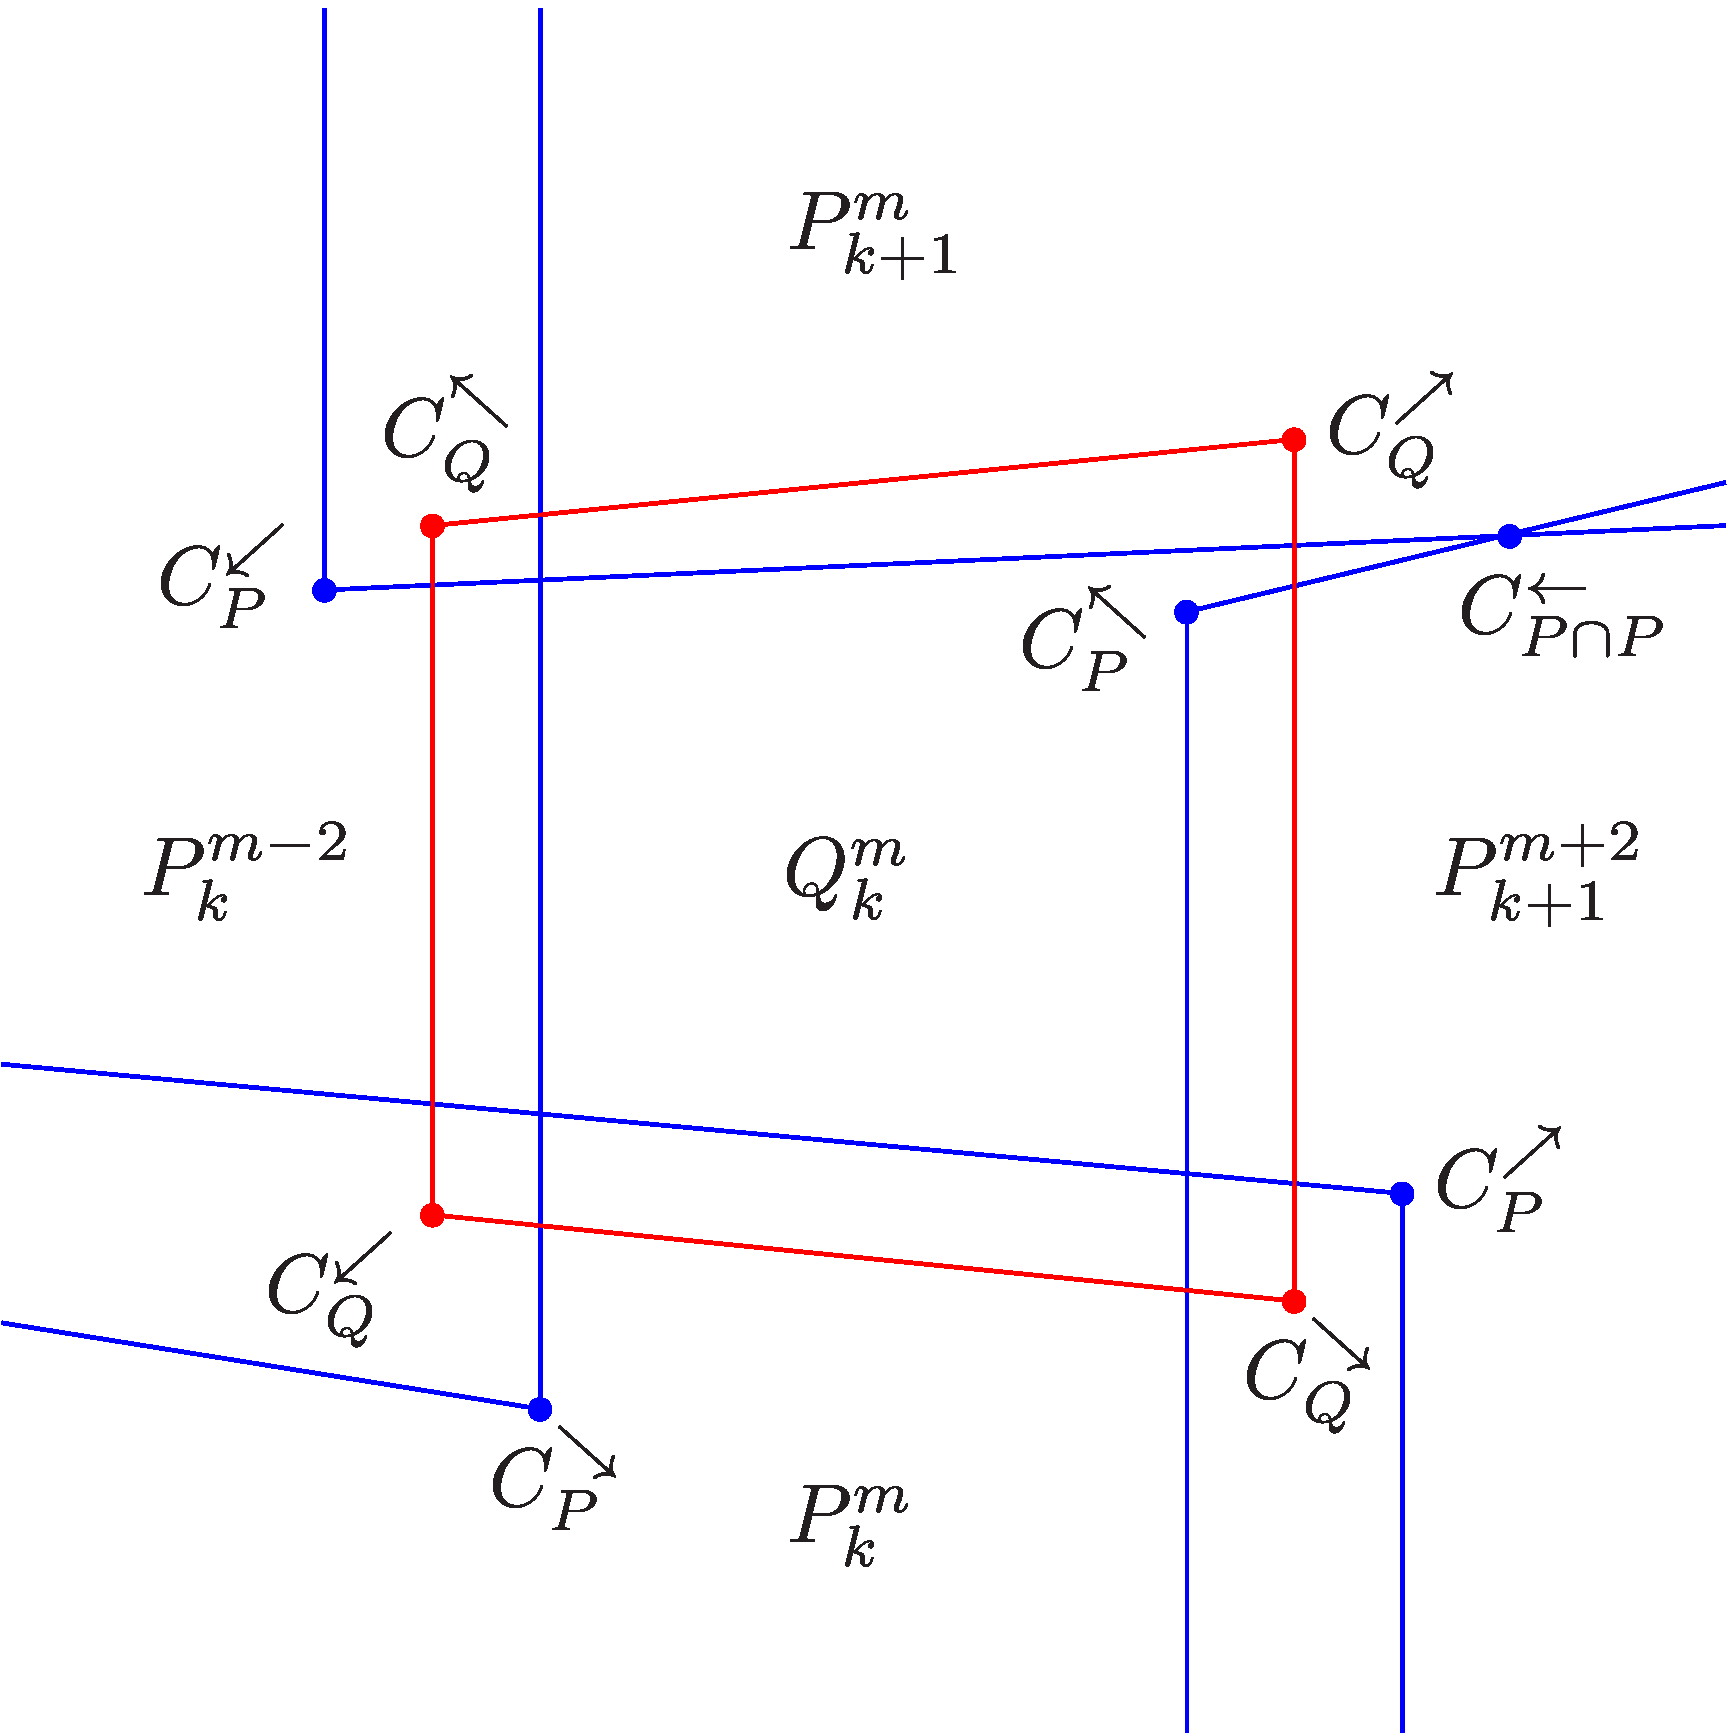
\includegraphics[width=.4 \textwidth]{../Figures/7/7.9b/result.png}
		\label{fig:add.change.schema.b}
	} \\
	\subfloat[]{
		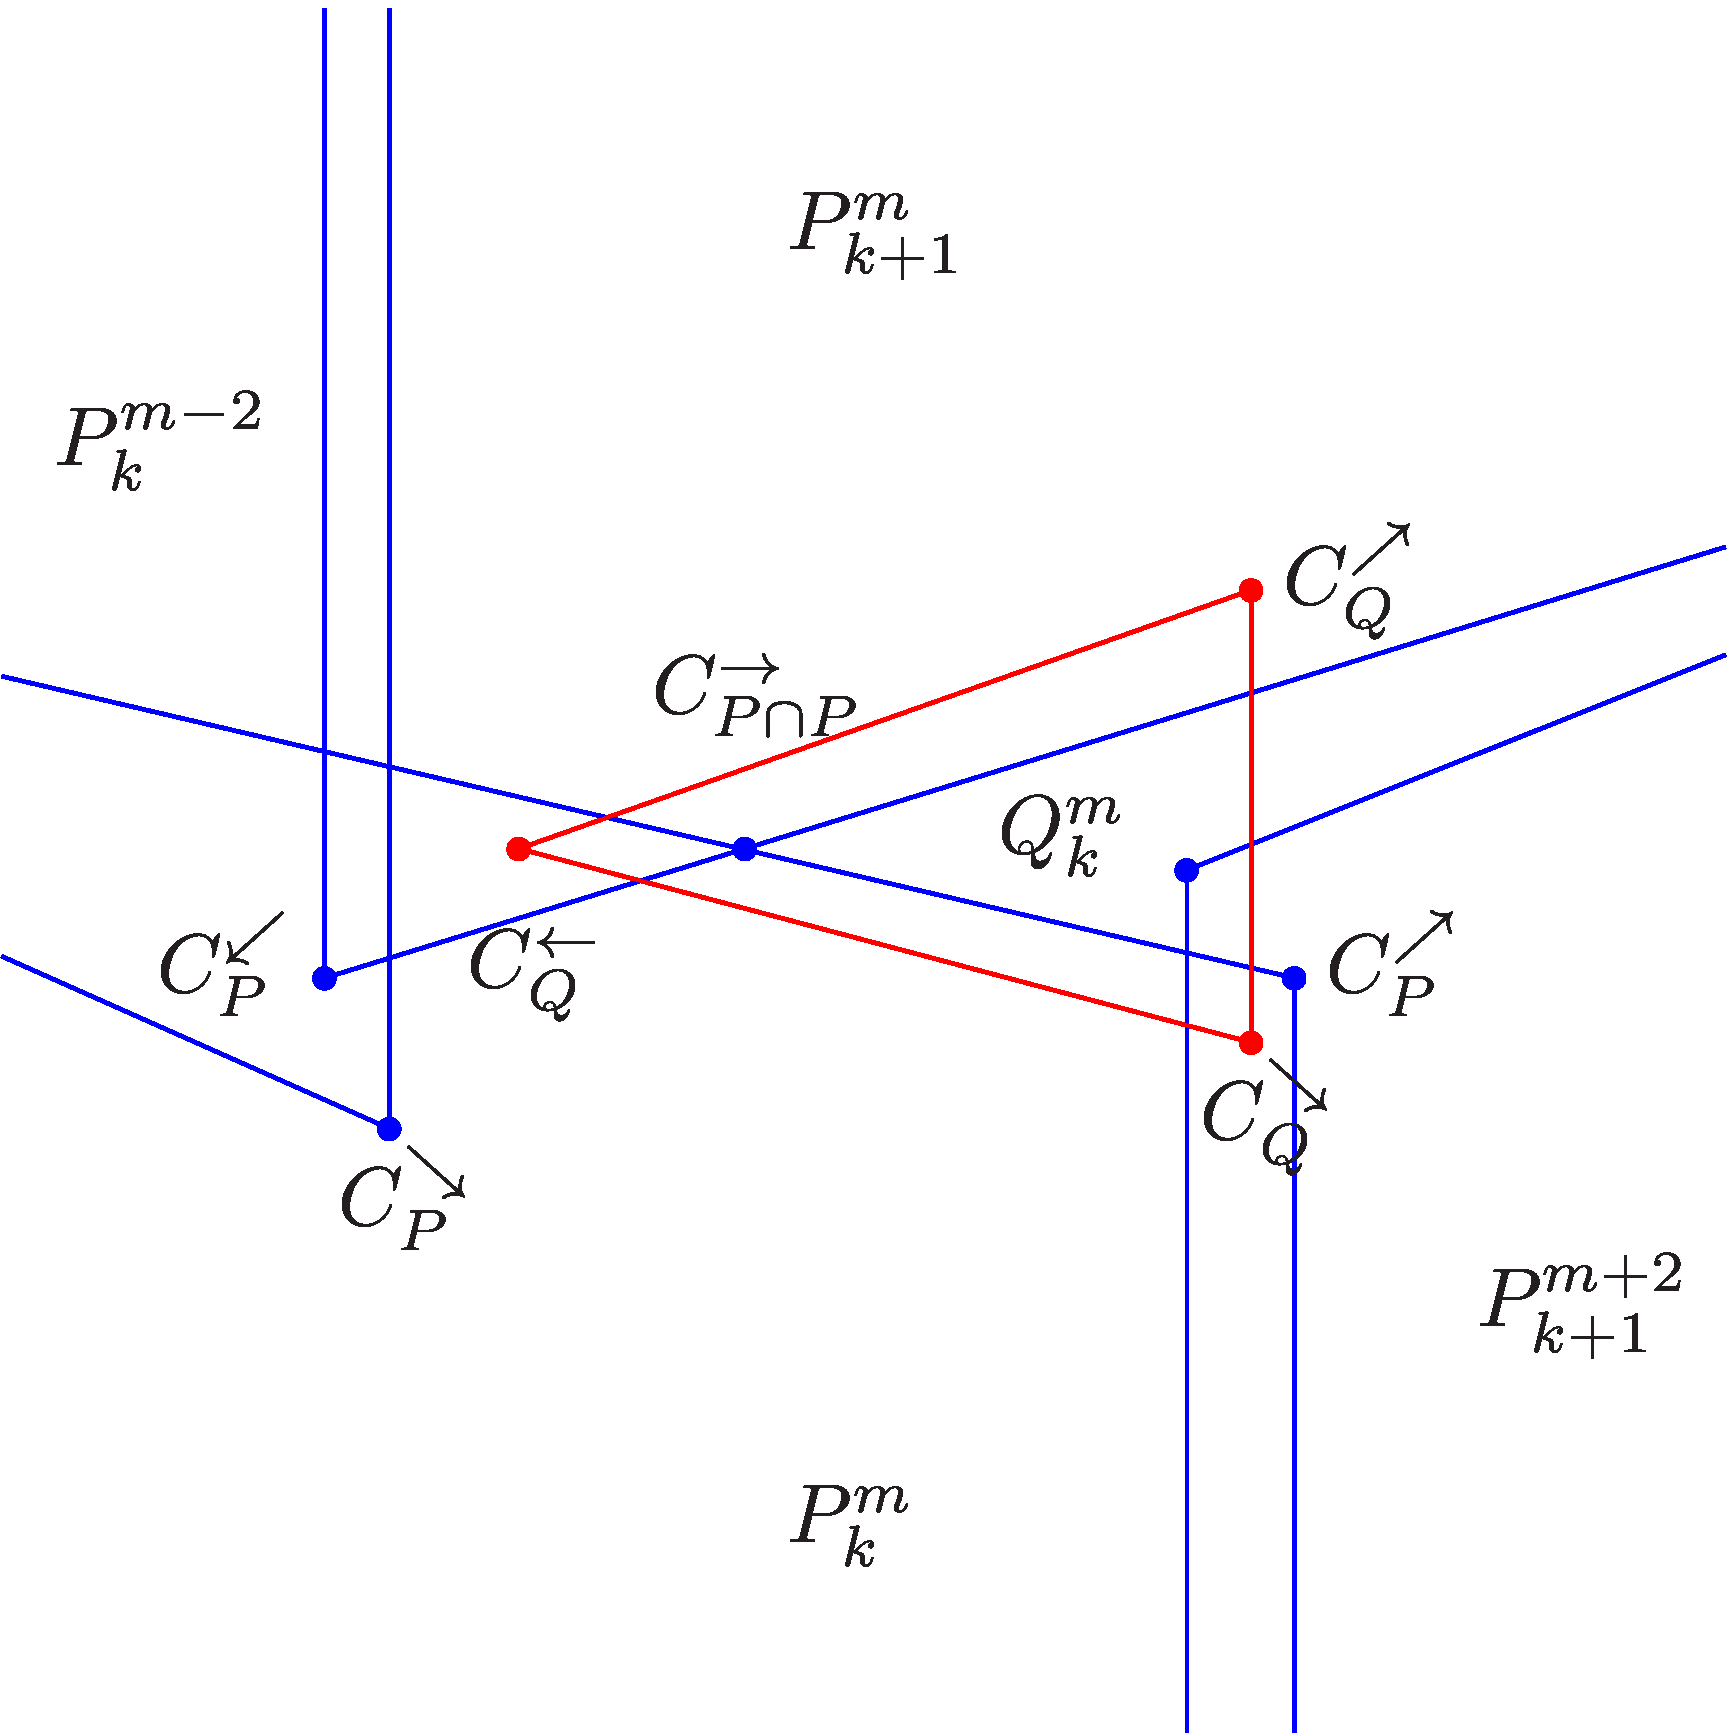
\includegraphics[width=.4 \textwidth]{../Figures/7/7.9c/result.png}
		\label{fig:add.change.schema.c}
	}
	\subfloat[]{
		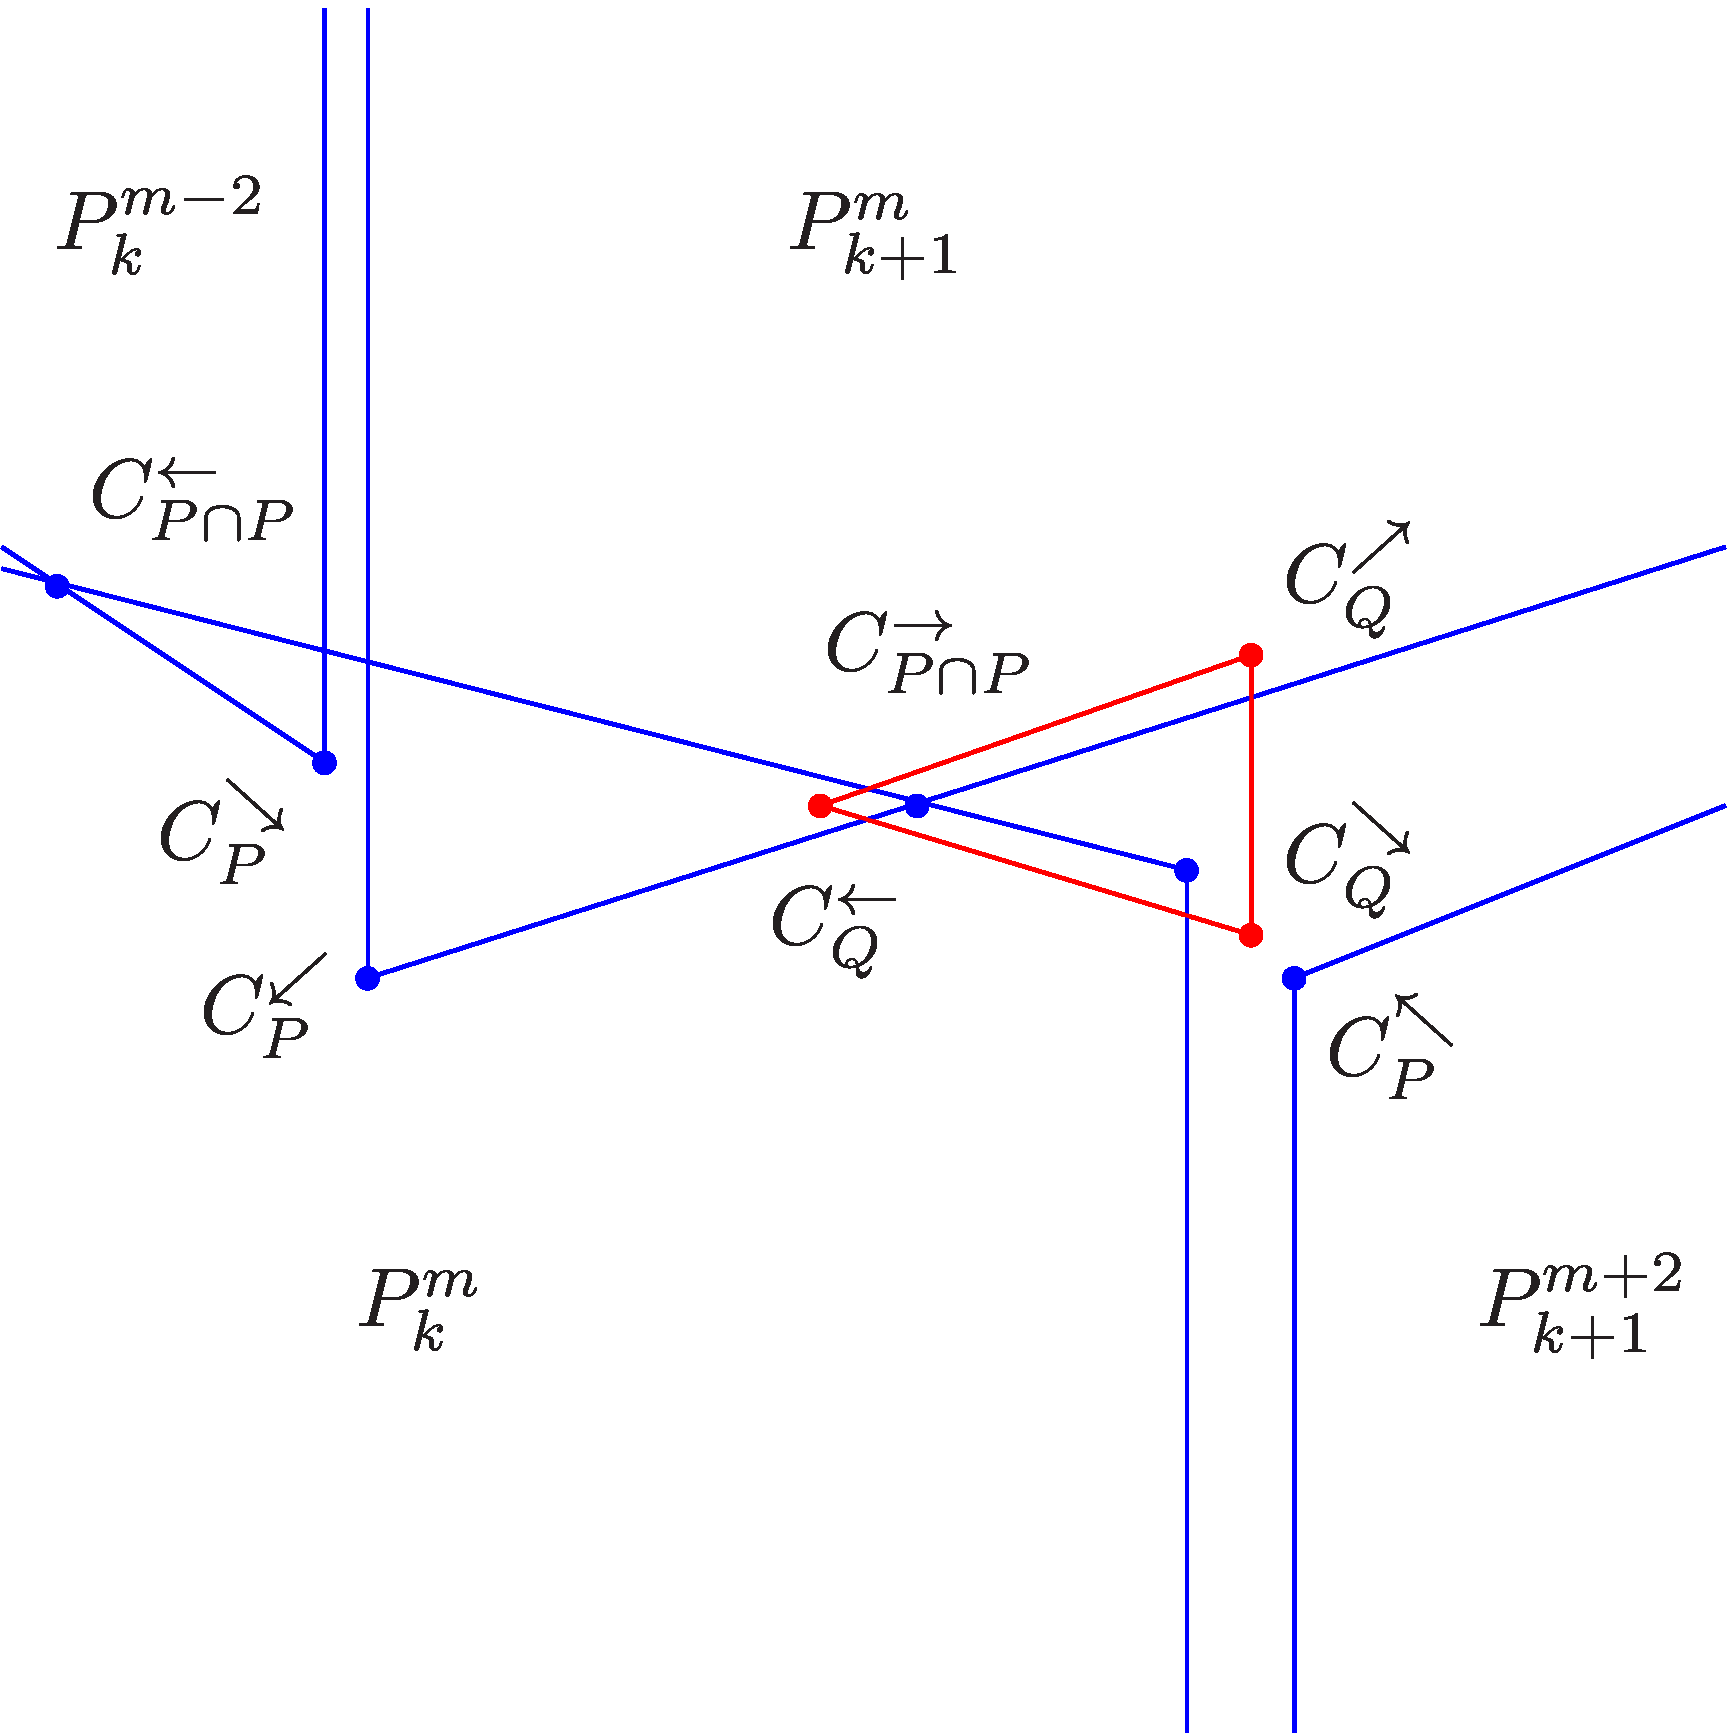
\includegraphics[width=.4 \textwidth]{../Figures/7/7.9d/result.png}
		\label{fig:add.change.schema.d}
	} \\
	\subfloat[]{
		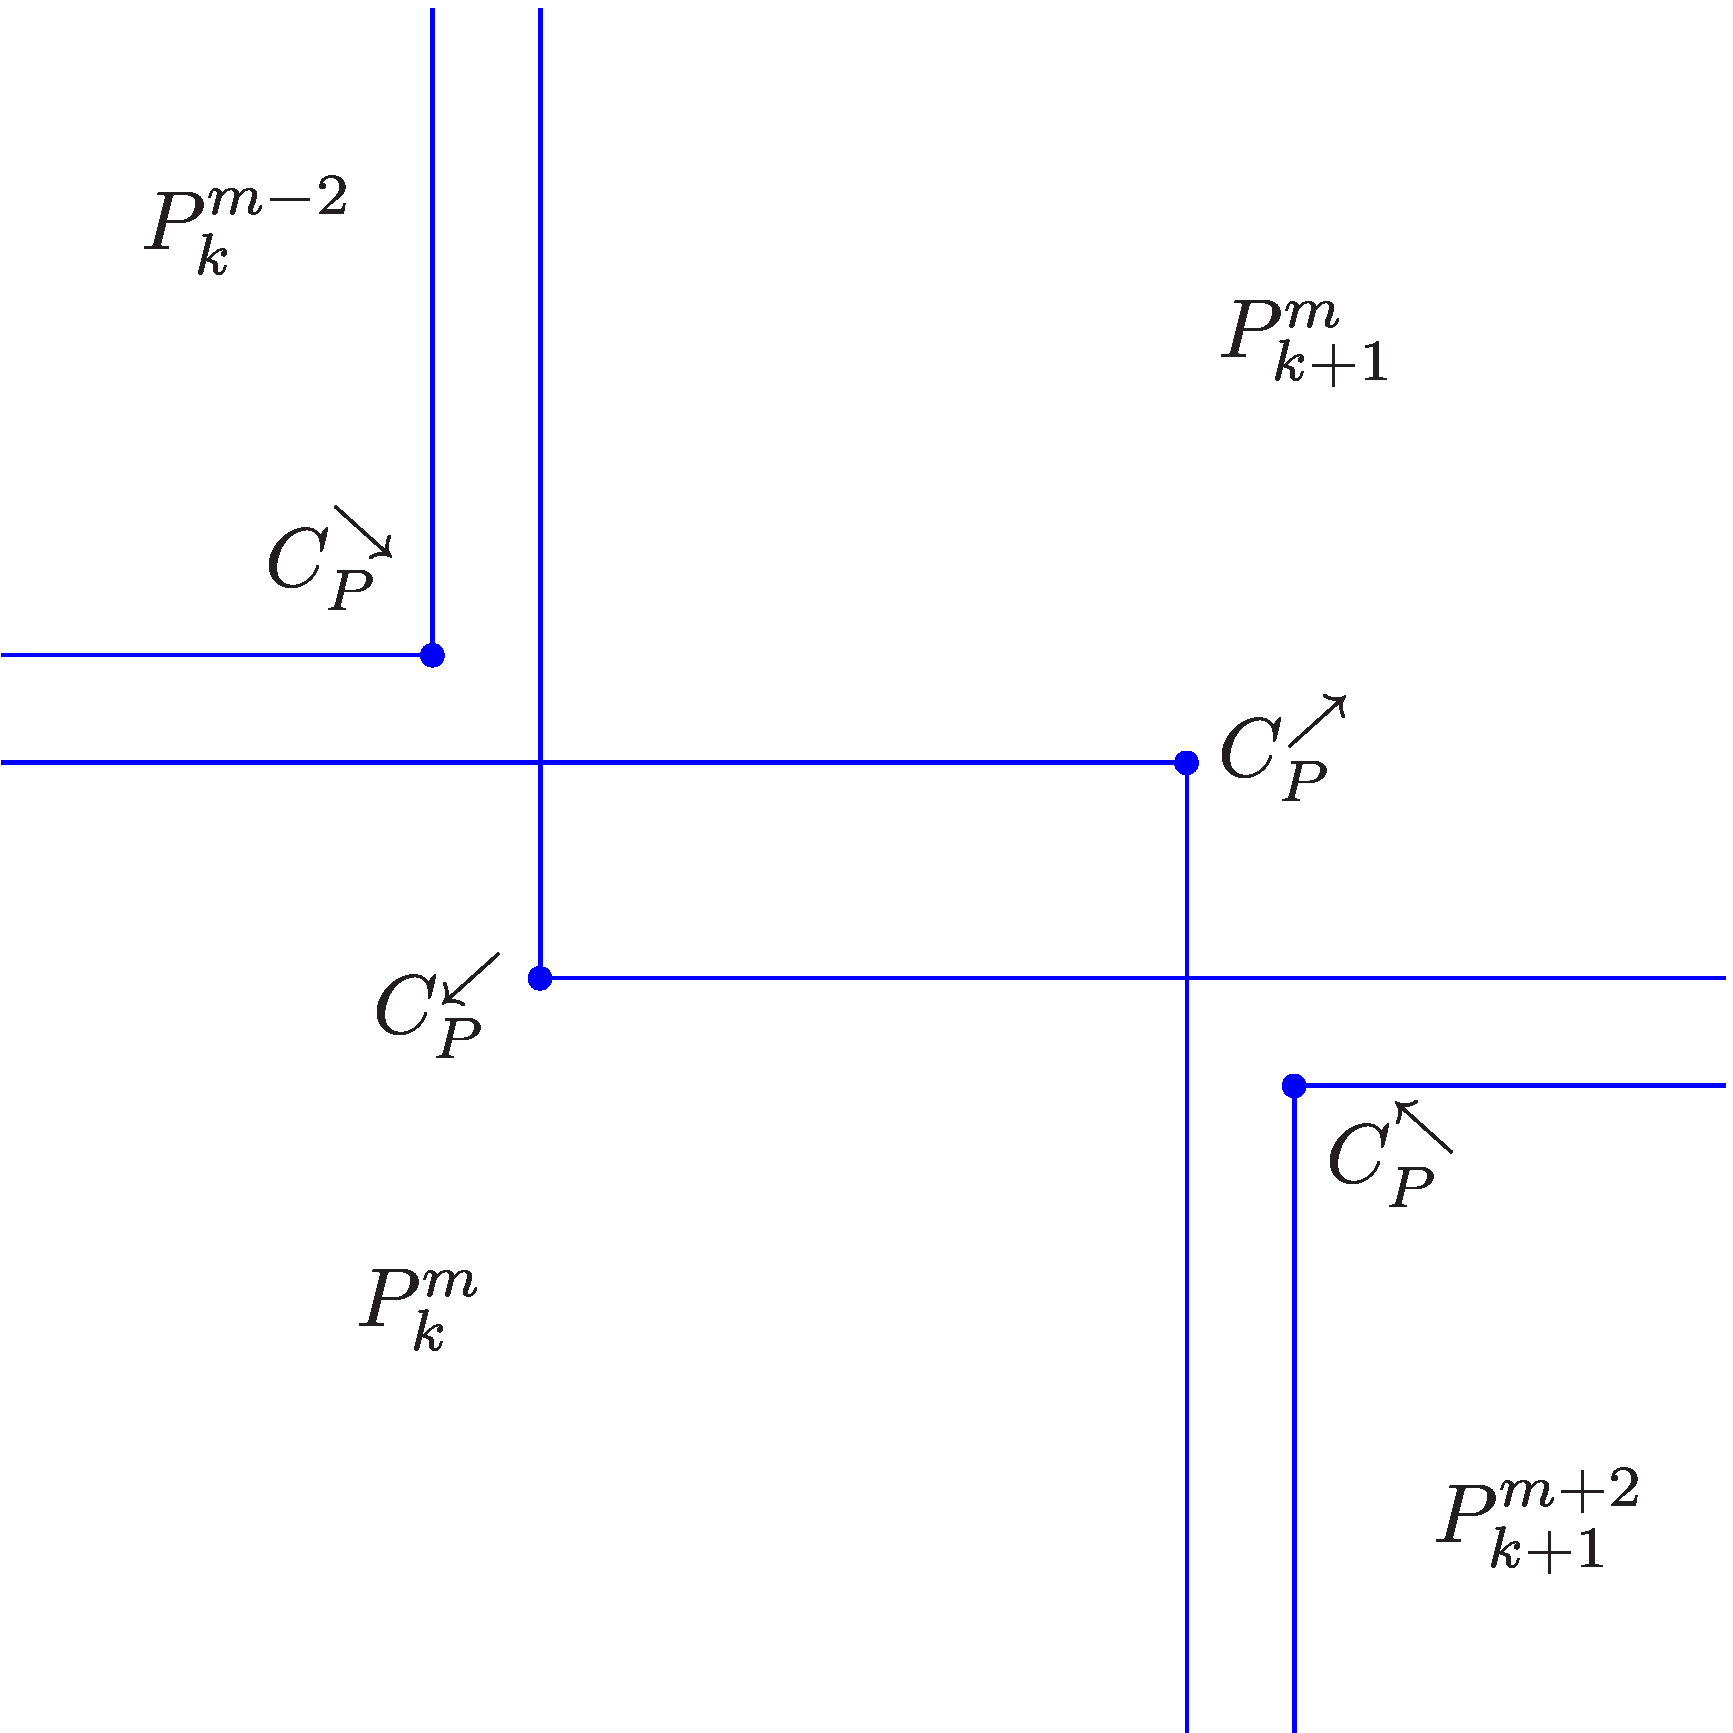
\includegraphics[width=.4 \textwidth]{../Figures/7/7.9e/result.png}
		\label{fig:add.change.schema.e}
	}
	\caption[Schematics of parameter region boundaries during the transformation of the archetypal model]{
		Schematics of parameter region boundaries during the transformation of the archetypal model.
		\todo{Adjust caption}
	}
	\label{fig:add.change.schema}
\end{figure}

\Cref{fig:add.change.schema} shows multiple schematics that are used in this section to summarize all changes.
All schematics show some boundaries of the ``type A'' parameter regions $P^m_k, P^{m-2}_{k-1}, P^m_{k+1},$ and $P^{m+2}_{k+1}$ and all boundaries of the ``type B'' parameter region $Q^m_k$.
The ``type B'' parameter region is in-between all the ``type A'' parameter regions in the beginning.
This is shown in \Cref{fig:add.change.schema.a}.
The corners of the parameter regions are marked as follows.
The upper right corner of the ``type B'' parameter region in the middle is marked with the point $C_Q^\nearrow$.
Similarly, the lower right corner is marked with the point $C_Q^\searrow$ and the remaining corners with the points $C_Q^\nwarrow$ and $C_Q^\nwarrow$.
The corners of the ``type A'' parameter regions are marked analogously with $C_P^\nearrow, C_P^\searrow, C_P^\nwarrow,$ and $C_P^\swarrow$.
But here, the corners belong to different parameter regions.

The changes are summarized in the order they happen to the parameter regions that are considered in the previous sections.
This order might differ for different parameter regions.

First, the upper left corner $C_Q^\nwarrow$ of the lower right ``type A'' parameter region $P^{m+2}_{k+1}$ moves down and crosses the lower boundary of the upper right ``type A'' parameter region $P^m_{k+1}$.
This is visible in \Cref{fig:add.change.schema.b}.
The point where the two boundaries of the horizontally neighboring ``type A'' parameter regions cross is marked as $C_{P \cap P}^\leftarrow$ because this point is now the only left corner point of the overlapping parameter region $P^{m+2}_{k+1} \cap P^{m}_{k+1}$.
For higher values of $b_L$, the point $C_Q^\nwarrow$ moves further down which causes the point where the boundaries cross to move right.
In \Cref{fig:add.change.schema.c}, this crossing point is not visible anymore, since it moved out of the domain of the picture.
In \Cref{fig:add.change.schema.d}, it is visible again, but on the left side of the schema.
Strictly speaking, this is not the same point but the left boundary of the overlapping parameter region $P^m_k \cap P^{m-2}_{k}$.
This point then collides with the corner point $C_P^\nearrow$ which then causes the two ``type A'' parameter regions to not overlap anymore.
This final scenario can be seen in \Cref{fig:add.change.schema.e}.
In the spaces that opened up between the vertically neighboring ``type A'' parameter regions, there are big hybrid parameter regions $\left[P^{m+2}_{k+1} \mid P^{m}_{k+1}\right]$ and $\left[P^m_k \mid P^{m-2}_k\right]$, respectively.
The hybrid parameter regions are not shown in the schematics but while the overlapping parameter regions have only three boundaries, they too only have three boundaries and are bounded to the right only by one codimension-2 point.
At this point, their upper and lower boundaries meet.

As we can see in the schematics, this change starts first and finishes last.
While the described process occurs, another change starts happening.
The points $C_P^\searrow$ and $C_Q^\nearrow$ move down while the points $C_Q\searrow$ and $C_P^\nearrow$ move up.
As soon as the point $C_P^\swarrow$ crosses the upper boundary of $P^m_k$, the ``type A'' parameter regions $P^m_k$ and $P^m_{k+1}$ start to overlap.
This overlapping region is bounded to the right only by the point where the horizontal boundaries of those two parameter regions cross.
This point is marked as $C_{P \cap P}^\rightarrow$ in \Cref{fig:add.change.schema.c}.
Also at some parameter values the corner points $C_Q^\nwarrow$ and $C_Q^\searrow$ of the ``type B'' parameter region $Q^m_k$ in the middle collide.
This creates a codimension-2 point that bounds the parameter region $Q^m_k$ to the left, hence it is marked as $C_Q^\leftarrow$.
Both these newly created corner points move right, as can be seen in \Cref{fig:add.change.schema.d}.
Finally, the corner point $C_{P \cap P}^\rightarrow$ collides with the corner point $C_P^\nearrow$ and the two horizontal boundaries of the ``type A'' parameter regions stop crossing.
The overlapping parameter region $P^m_k \cap P^m_{k+1}$ is now bounded by four boundaries, as can be seen in \Cref{fig:add.change.schema.e}.
And the corner point $C_Q^\leftarrow$ crosses the right boundary of the ``type B'' parameter region, destroying the ``type B'' parameter region.

While that change is happening, one more change takes place.
This change does not happen by two boundaries crossing at one point like the last two changes.
Instead, the numeric evidence suggests that it happens at once.
The corner point $C_P^\nwarrow$ crosses the right boundary of $P^m_k$ at the same time, the lower right corner point of $P^{m}_{k}$ which is not pictured here crosses the left boundary of $P^{m+2}_{k+1}$.
This lower corner point is not pictured, but the lower right corner point of $P^{m-2}_k$ is pictured and marked as $C_P^\searrow$.
Here, the equivalent happens for the horizontally neighboring ``type A'' parameter regions $P^{m-2}_k$ and $P^m_{k+1}$.
In \Cref{fig:add.change.schema.c}, the horizontally neighboring ``type A'' parameter regions overlap and in \Cref{fig:add.change.schema.d}, the parameter regions do not overlap.
Instead, there is now space in-between the horizontally neighboring ``type A'' parameter regions.
In this space there now is a big hybrid parameter region and \gls{pal} structures, similar to the vertically neighboring ``type A'' parameter regions.

\subsubsection{Observations}

The local minima on branches $f_\A$ and $f_\C$ seem to be important for the ``type B'' parameter regions.
That means, parameter regions with coexisting asymmetrical cycles with the \textbf{same} period.
At the same time, these minima seem to prevent period-adding structures.
It will be proven next that ``type B'' parameter regions are impossible with only increasing branches.

\begin{lemma}[Number and Positions of Points of two Cycles on an Increasing Branch]
	Let $f_\X$ be an increasing branch of some model function $f$.
	If two cycles $\sigma_1$ and $\sigma_b$ have points on this branch, there are two possibilities for the relative number of points and relative position of the points.
	\begin{enumerate}
		\item Both cycles have the same number of points on the branch $f_\X$.
		      Let the first point of $\sigma_1$ be to the left of the first point of $\sigma_2$ on this branch w.l.o.g.
		      Then the last point of $\sigma_1$ is also to the left of the last point of $\sigma_2$ on this branch.
		      \Cref{fig:add.change.increasing.a} illustrates this case.
		\item One cycle has one more point on the branch $f_\X$.
		      Let $\sigma_1$ be the cycle with more points on this branch w.l.o.g.
		      Then the first point of $\sigma_1$ is to the left of the first point of $\sigma_2$ on this branch and the last point of $\sigma_1$ is to the right of the last point of $\sigma_2$ on this branch.
		      \Cref{fig:add.change.increasing.b} illustrates this case.
	\end{enumerate}
	\label{lemma:add.num.pos.points.increasing}
\end{lemma}

\begin{figure}
	\centering
	\subfloat[Same number of points]{
		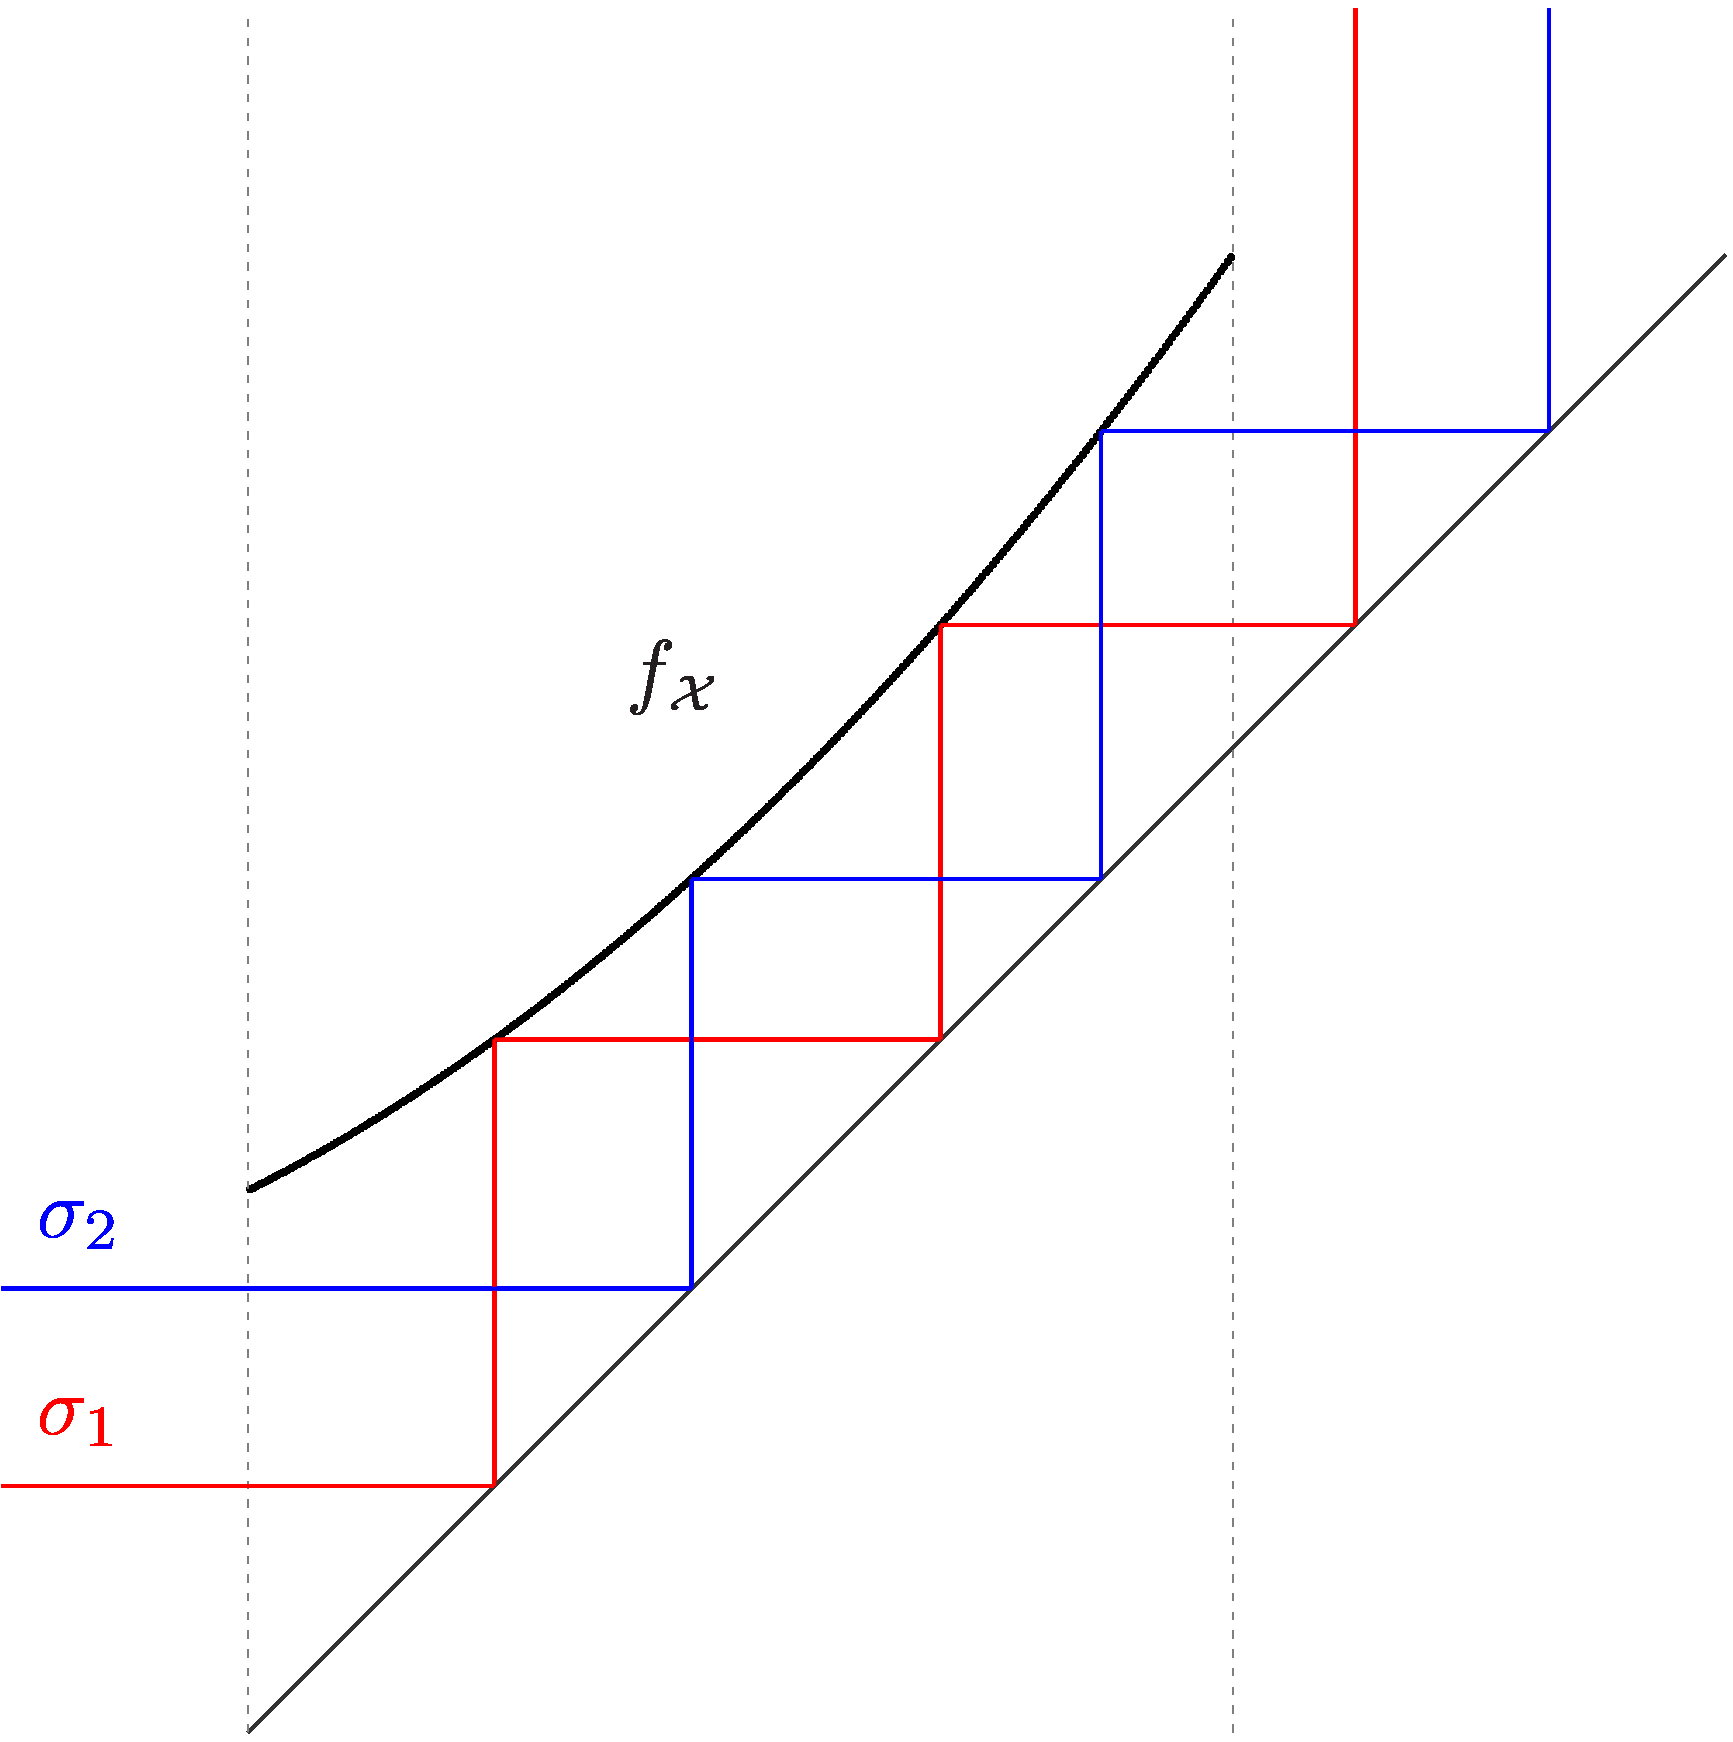
\includegraphics[width=.35 \textwidth]{../Figures/7/7.10a/result.png}
		\label{fig:add.change.increasing.a}
	} \quad
	\subfloat[Number of points differing by one]{
		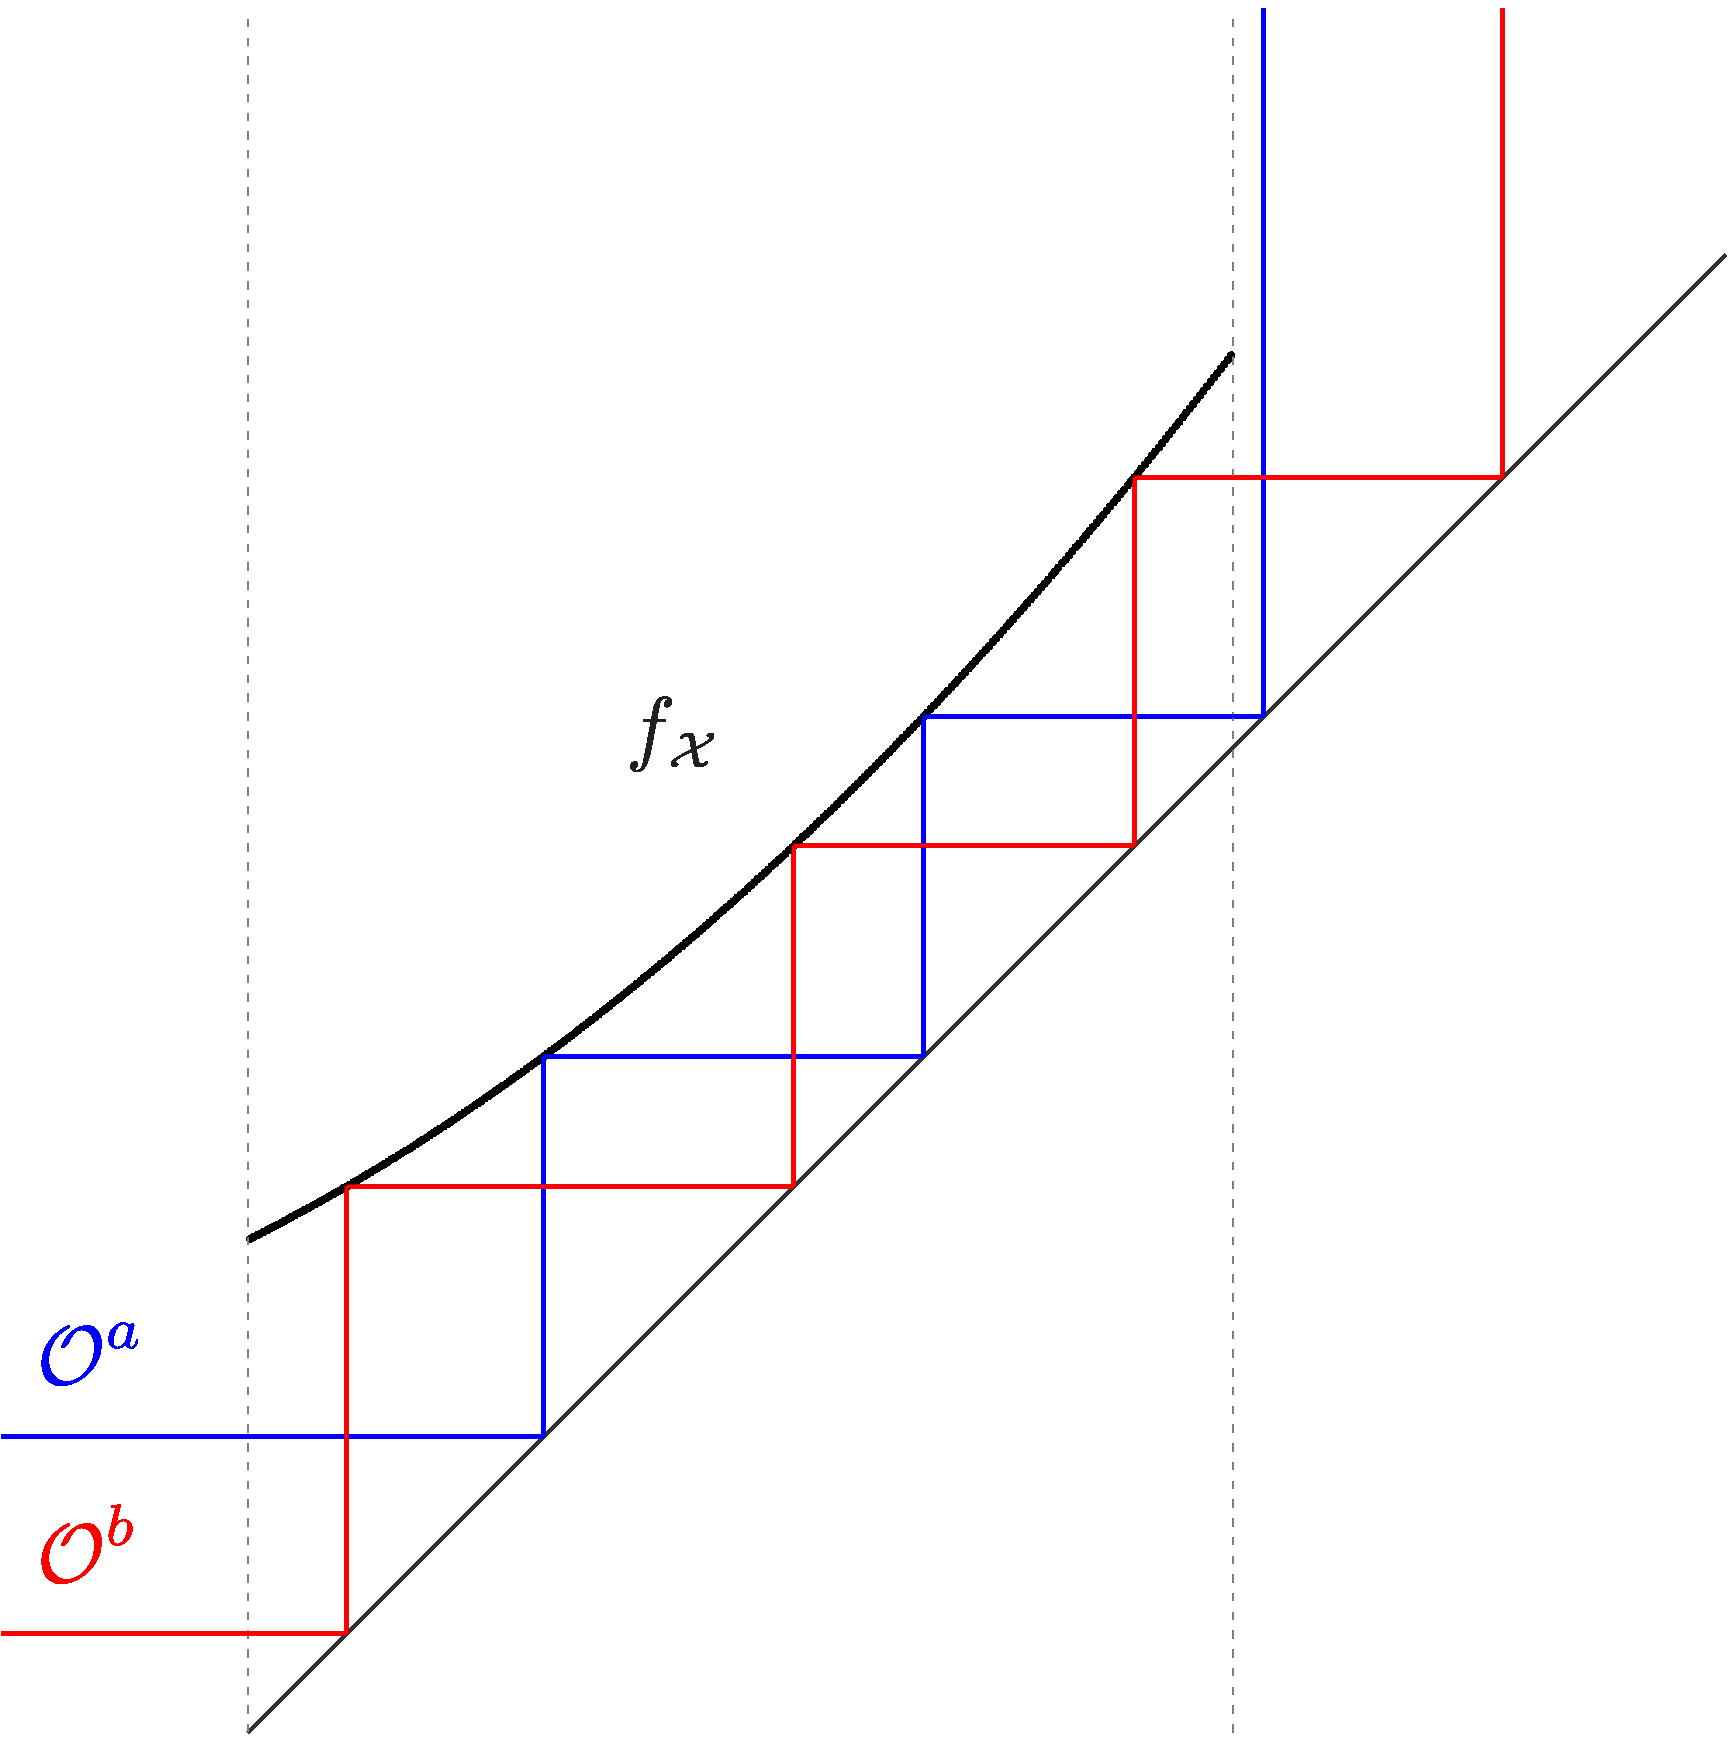
\includegraphics[width=.35 \textwidth]{../Figures/7/7.10b/result.png}
		\label{fig:add.change.increasing.b}
	}
	\caption[Illustration of relative number and positions of points of two cycles on an increasing branch]{
		Illustration of relative number and positions of points of two cycles on an increasing branch.
		Both figures show a function branch $f_\X$ and parts of two cycles, $\sigma_1$ shown in red and $\sigma_2$ shown in blue.
		(a) shows the case where both cycles have the same number of points on the branch $f_\X$ and the first point of $\sigma_1$ is to the left of the first point of $\sigma_2$ on this branch.
		(a) shows the case where the cycle $\sigma_1$ has one point more on the branch $f_\X$ than $\sigma_2$ and the first point of $\sigma_1$ is to the left of the first point of $\sigma_2$ on this branch.
	}
	\label{fig:add.change.increasing}
\end{figure}

\begin{theorem}[No ``Type B'' Parameter Regions with only Increasing Branches]
	The ``type B'' parameter regions are not possible in the increasing archetypal model.
	The minima on the branches $f_\A$ and $f_\C$ are essential for the bifurcation structure.
\end{theorem}

\begin{proof} \phantom{x} \\
	Let's assume that all branches of the archetypal model $f_\A, f_\B, f_\C,$ and $f_\D$ are increasing.
	And let $\sigma_1$ and $\sigma_2$ be ``type B'' twin cycles.
	The following conditions are true for such cycles.
	\begin{subequations}
		\begin{align}
			|\sigma_1|_\A - 1 & = |\sigma_2|_\A \label{equ:add.change.conseq.sigmaA} \\
			|\sigma_1|_\B + 1 & = |\sigma_2|_\B \label{equ:add.change.conseq.sigmaB} \\
			|\sigma_1|_\C + 1 & = |\sigma_2|_\C \label{equ:add.change.conseq.sigmaC} \\
			|\sigma_1|_\D - 1 & = |\sigma_2|_\D \label{equ:add.change.conseq.sigmaD}
		\end{align}
	\end{subequations}

	For \Cref{equ:add.change.conseq.sigmaA} to hold, the first point of  $\sigma_1$ needs to be to the left of first point of  $\sigma_2$ on the branch $f_\A$, because  $\sigma_1$ has one point more on this branch than  $\sigma_2$ and this branch is increasing.
	At the same time, the last point of  $\sigma_1$ must be to the right of the last point of  $\sigma_2$ on this branch.

	The order of the first points on the next branch, $f_\B$, is the same as for the last points on the branch $f_\A$.
	So the first point of  $\sigma_2$ is to the left of the first point of  $\sigma_1$ on this branch.
	For \Cref{equ:add.change.conseq.sigmaB} to hold, the last point of  $\sigma_2$ must be to the right of the last point of  $\sigma_1$ on this branch per the same logic as before.

	The order of the first points on the next branch, $f_\C$, is the same as for the last points on the branch $f_\B$.
	So the first point of  $\sigma_1$ is to the left of the first point of  $\sigma_2$ on this branch.
	This is a contradiction, since the first point of  $\sigma_1$ on the branch $f_\A$ is also to the left of the first point of  $\sigma_2$ on that branch.
	This violates the symmetry.
	Also, \Cref{equ:add.change.conseq.sigmaC} cannot be fulfilled if the first point of  $\sigma_1$ is to the left of the first point of  $\sigma_2$ on the branch $f_\C$, since the first point of  with more points, $\sigma_2$ in this case, on the branch must be to the left of the first point of the other cycle on that branch if the branch is increasing.
	\hfill $\blacksquare$
\end{proof}
